In the following subsection, we list the different properties and lemmas that are useful to the proofs of the convergence of algorithm \ref{FedAVG}. First, we consider convexity and smoothness lemmas: 

\begin{figure}[h!]
    \centering
    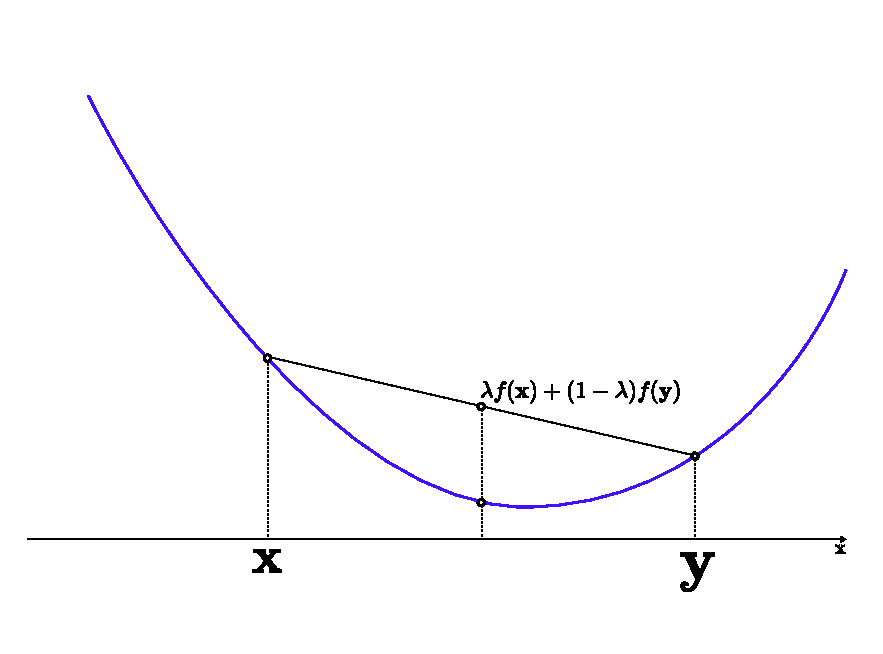
\includegraphics[width=0.5\textwidth]{figures/convexity.pdf}
    \caption{Visual illustration of convexity.}
\end{figure}

\begin{property}
    (Convexity) consider a real value function $f:\bm{dom}(f)\rightarrow \mathbb{R}$, we say that $f$ if 
    \begin{enumerate}
        \item $\bm{dom}(f)$ is convex
        \item $\forall \bm{x},\bm{y} \in \bm{dom}(f)$ we have: 
        \[ f(\lambda \bm{x} + (1-\lambda) \bm{y}) \leq \lambda f(\bm{x}) + (1-\lambda) f(\bm{y}). \]
    \end{enumerate}
    \label{chord_convexity}
\end{property}


\begin{property}
    (First order characterization of convexity) suppose $\bm{dom}(f)$ is open and that $f:\bm{dom}(f) \rightarrow \mathbb{R}$ is differentiable (it's gradient $\nabla f(x)$ exists $\forall \bm{x} \in \bm{dom}(f)$), then $f$ is convex $\iff$
    \[ f(\bm{y}) \geq f(\bm{x}) + \langle \nabla f(\bm{x}) , \bm{y}-\bm{x} \rangle ,~  \forall \bm{x},\bm{y} \in \bm{dom}(f). \]
    \label{convexity}
\end{property}
\noindent


Here a geometrical interpretation of convexity which is useful, convexity implies that the segment between any two points in the domain passes above the function $f$. This implies the following observation:
\begin{observation}
    For $f:\bm{dom}(f) \rightarrow \mathbb{R}$ convex, we have the following property. Any hyperplane parallel to the hyperplane tangent to $f$ in $\bm{x}$ which intersects $f$ on some point $\bm{z}$ in $\bm{dom}(f)$ is "above" the tangent hyperplane, more rigorously:
    \begin{align*}
        f(\bm{x}) + \langle \nabla f(\bm{x}), \bm{y}-\bm{x} \rangle \geq  f(\bm{z}) + \langle \nabla f(\bm{x}), \bm{y}-\bm{z} \rangle, ~  \forall \bm{x},\bm{y} ,\bm{z} \in \bm{dom}(f). 
    \end{align*}
    \label{obs}
\end{observation}

\begin{figure}[h!]
    \centering
    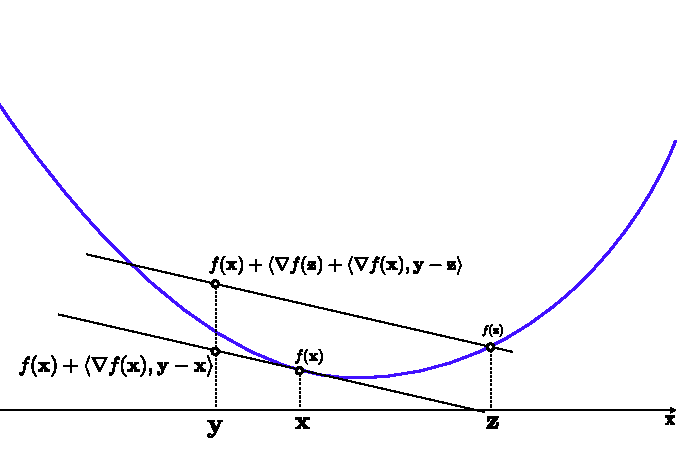
\includegraphics[width=0.5\textwidth]{figures/observation.pdf}
    \caption{Visual illustration of observation \ref{obs}.}
\end{figure}


\noindent
We will also use the definition of L-smoothness:
\begin{property}
    (L-Smoothness) let $f:\bm{dom}(f) \rightarrow \mathbb{R}$ be a differentiable function and $X \subseteq \bm{dom}(f)$ convex and $L\in\mathbb{R}_+$. Function $f$ is called \textit{smooth} over $X$ if:
    \[  f(\bm{y}) \leq f(\bm{x}) +  \langle \nabla f(\bm{x}) , \bm{y}-\bm{x} \rangle +  \frac{L}{2} \|\bm{y}-\bm{x} \|^2 ,~  \forall \bm{x},\bm{y} \in \bm{dom}(f). \]
    \label{lsmooth}
\end{property}

\noindent
Next we look at a geometric identity: the parallelogram law:

\begin{property}
    (Polarization identity) let $a,b \in \mathbb{R}^d$ be two vectors, let $\|\cdot\|$ denote their $2$-norm and $\langle a , b \rangle$ denote the inner (dot) product. Then the following equality is true:
    \[  \langle a , b \rangle =  \frac{1}{2}\| a+b\|^2 - \|a\|^2- \|b\|^2 = \frac{1}{2}  \|a\|^2 + \|b\|^2 - \| a-b\|^2.  \]
    \label{polID}
\end{property}

\begin{property}
    (Young's inequality) let $a,b \in \mathbb{R}^d$ be two vectors, let $\|\cdot\|$ denote their $2$-norm and $\langle a , b \rangle$ denote the inner (dot) product and $\lambda \in \mathbb{R}^+$, the following inequality is true:
    \[  \langle a , b \rangle \leq \frac{\lambda^2}{2} \| a \|^2 + \frac{1}{2 \lambda^2} \| b \|^2. \]
    \label{young}
\end{property}

